\section{Alit Fajar Kurniawan(1174057)}
\subsection{cara instalasi Map Server dan Map Proxy}
Web Service yang digunakan pada map server ini adalah ms4w yang dapat didownload dari \href{https://ms4w.com/download.html#download}{Link download instaler MS4W}.

cara-cara menginstall map server dan maproxy.
\begin{enumerate}
    \item pertama kalian bisa membuka link yang telah saya sediakan diatas, kemudian bisa memilih installer yang berformat .exe , atau kalian bisa juga mendownload yang file zip. jika menggunakan yang file zip maka kalian tidak perlu lagi mengubah settingan ketika menginstallnya dan semua file sudah tersedia
    \hfill\break
	\begin{figure}[H]
		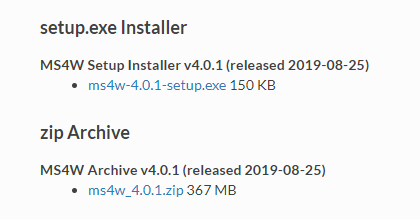
\includegraphics[width=8cm]{figures/1174057/4Tugassatu.png}
		\centering
		\caption{Download File MS4W}
	\end{figure}

	\item selanjutnya, buka file installer yang telah di download
    \hfill\break
	\begin{figure}[H]
		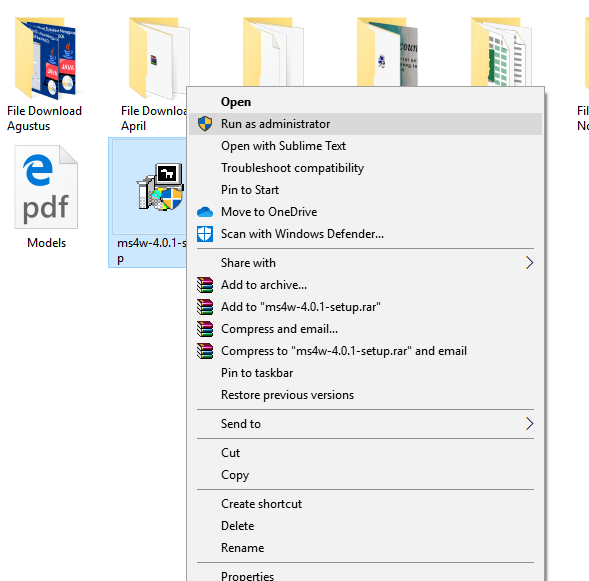
\includegraphics[width=8cm]{figures/1174057/4Tugasdua.PNG}
		\centering
		\caption{Membuka Installer}
	\end{figure}

	\item selanjutnya bisa langsung next next saja, dan jangan lupa mengubah port nya menjadi 8080.

	\item kemudian akan muncul proses seperti dibawah ini, dan tunggu saja
    \hfill\break
	\begin{figure}[H]
		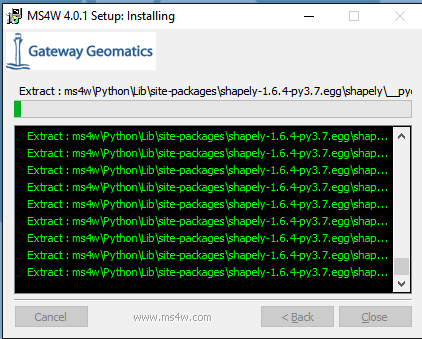
\includegraphics[width=8cm]{figures/1174057/4Tugastiga.PNG}
		\centering
		\caption{Proses instalasi 1}
	\end{figure}

	\begin{figure}[H]
		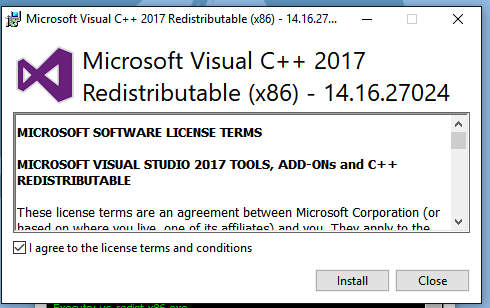
\includegraphics[width=8cm]{figures/1174057/4Tugasempat.PNG}
		\centering
		\caption{Proses instalasi 2}
	\end{figure}

	\item setelah melakukan instalasi, selanjutnya bisa membuka MS4W shell yang terdapat pada dekstop
    \hfill\break
	\begin{figure}[H]
		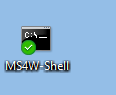
\includegraphics[width=8cm]{figures/1174057/4Tugaslima.PNG}
		\centering
		\caption{Membuka Commadline}
	\end{figure}

	\item kemudian kita memeriksa mapserver yang telah diinstall dengan cara mengetikkan "mapserv -v"
    \hfill\break
	\begin{figure}[H]
		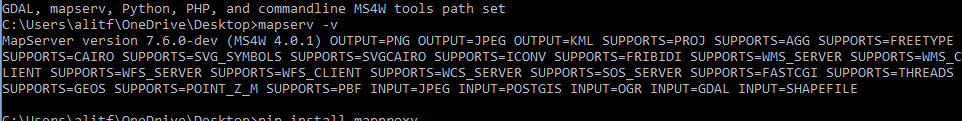
\includegraphics[width=8cm]{figures/1174057/4Tugasenam.PNG}
		\centering
		\caption{Cek Map Server}
	\end{figure}

	\item jika sudah muncul seperti gambar di atas berarti Map Server telah terinstall

	\item kita juga bisa mengeceknya pada chrome dan membuka "localhost:8080"
	\begin{figure}[H]
		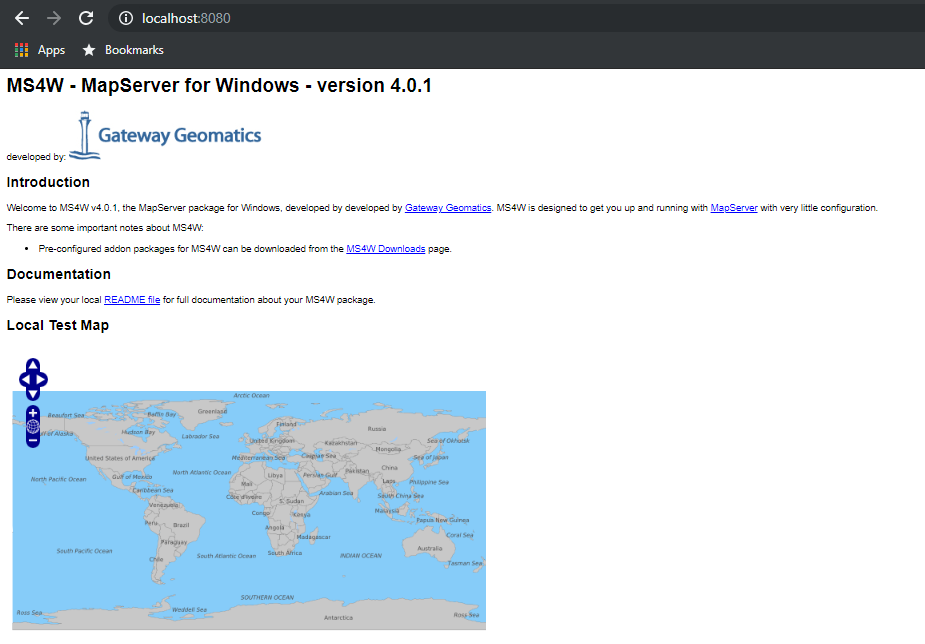
\includegraphics[width=8cm]{figures/1174057/4Tugastujuh.PNG}
		\centering
		\caption{Cek Map Server}
	\end{figure}

	\item selanjutnya kita akan menginstall Map Proxy pada commandline MS4W shell, dengan cara mengetikkan "pip install mapproxy"
	\begin{figure}[H]
		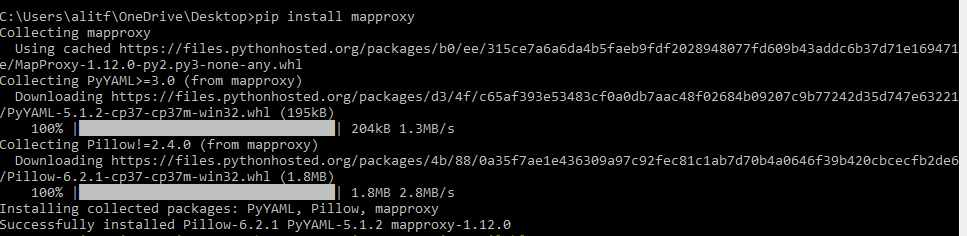
\includegraphics[width=8cm]{figures/1174057/4Tugaslapan.PNG}
		\centering
		\caption{Install Map Proxy}
	\end{figure}

	\item tunggu sampai selesai. dan proses instalasi map server dan map proxy telah selesai.
\end{enumerate}

\subsection{Video Tutorial Install Map server dan Map Proxy}
\href{https://youtu.be/-cprZtvh7yU}{Link Youtube say}
